\subsection{The F$_s$ helical peptide.}
\label{applications:helix}

% TODO:

% TWO-COLUMN TABLE OF STATES FOR ALPHA HELIX
\newcommand*{\DOT}{.}
\newcommand{\colpdbwidth}{0.75in}
\newcommand{\pdbfigcol}[1]{\parbox{\colpdbwidth}{\includegraphics[width=\colpdbwidth]{#1}}}
\newcommand{\pdbimg}[1]{\pdbfigcol{chapters/automatic-state-decomposition/figures/alpha-helix/state-pdbs/10\DOT ensemble-merged-#1.png}}
\begin{table*}[tb]
\caption{{\bf Macrostates from a 20-state state decomposition of the F$_s$ helical peptide.}  The backbone is depicted in alpha carbon trace, and arginine sidechains are shown in blue (Arg10), magenta (Arg15), and green (Arg20) for clarity.}
\label{table:helix-states}
\begin{center}
\begin{tabular}{ccccccccc}
\hline
state & 1 & 2 & 3 & 4 & 5\\
& \pdbimg{143215} & \pdbimg{116359} & \pdbimg{509002} & \pdbimg{344096} & \pdbimg{118439} \\
members & 358 712 & 98 222 & 46 921 & 22 559 & 22 367 \\
$\tau_\mathrm{ac}$ (ns) & 3.1 & 0.9 & 1.4 & 0.6 & 4.0 \\
\hline
state & 6 & 7 & 8 & 9 & 10 \\
&  \pdbimg{544652} & \pdbimg{189995} & \pdbimg{439117} & \pdbimg{514253} & \pdbimg{607324} \\
members & 15 859 & 11 975 & 11 053 & 11 024 \\
$\tau_\mathrm{ac}$ (ns) & 1.3 & 1.6 & 2.2 & 2.0 \\
\hline
state  & 11 & 12 & 13 & 14 & 15 \\
 & \pdbimg{532115} & \pdbimg{16278} & \pdbimg{618465} & \pdbimg{438247} & \pdbimg{509683} \\
members & 7 976 & 7 808 & 7 771 & 5 978 & 5 626 \\
$\tau_\mathrm{ac}$ (ns) & 2.2 & 1.2 & 1.6 & 11.3 & 2.3 \\
\hline
state  & 16 & 17 & 18 & 19 & 20 \\
& \pdbimg{257470} & \pdbimg{348373} & \pdbimg{503295} & \pdbimg{484545} & \pdbimg{596094} \\
members & 1 856 & 955 & 531 & 525 & 490 \\
$\tau_\mathrm{ac}$ (ns) & 5.0 & 10.3 & 47.0 & 29.1 & 15.2 \\
\hline
\end{tabular}
\end{center}
\end{table*}

To illustrate behavior of the automatic state decomposition method on a larger peptide system with fast kinetics, we applied it to the 21-residue helix-forming F$_s$ peptide, which has been studied extensively both experimentally \cite{lockhart:science:1992,lockhart:science:1993,williams:biochem:1996,eaton:biochem:1997,lednev:jacs:2001} and computationally \cite{garcia:2002a,duan:jpcb:2004,sorin:2005a,sorin:2005b}.
Since helix formation occurs on the nanosecond timescale, Sorin \emph{et al.}\ were able to reach equilibrium from both helix and coil conformations and observe equilibrium conformational dynamics using ensembles of molecular dynamics trajectories on the distributed computing platform Folding@Home \cite{sorin:2005b}.
Two sets of 1000 trajectories at 302 K of varying length of the capped F$_s$ peptide (sequence Ace-A$_5$[AAARA]$_3$A-Nme), one set initiated from an ideal helix and another from a random coil, were obtained from Sorin \emph{et al.}\cite{sorin:2005b}; details of the simulation protocol are available therein.
The first 40 ns of each trajectory, a conservative overestimate of the time to reach equilibrium from either helix or coil, was discarded, and the two sets of trajectories combined to yield a total of 1689 trajectories varying in length from 10 ns to 95 ns with a sampling interval of 100 ps.
In total, this equilibrium dataset contained nearly 65 $\mu$s of simulation data in 642 604 conformations.
The peptide was modeled using the AMBER-99$\phi$ forcefield \cite{AMBER-parm99,sorin:2005b} and solvated in TIP3P water \cite{jorgensen:1983a}.
Though the Berendsen weak-coupling scheme \cite{berendsen:1984a} was employed for thermal and pressure control\footnote{We note that thermal and pressure control, by design, modulate the velocities of molecules in the system, which may have a nonphysical effect on dynamics.  In this particular application, however, we are only comparing our analysis with the original simulation data, rather than directly with experiment.}, we presume the trajectories still obey microscopic reversibility when only the coordinates of the macromolecular solute are considered for the purposes of computing transition probabilities.

We performed automatic state decomposition on this dataset to generate a set of 20 macrostates through 10 iterations of splitting and lumping.
In the first iteration, the sampled region of conformation space was split into 400 microstates.
In subsequent iterations, each macrostate was split into 50 microstates (or, if the expected microstate size would fall below 500 configurations, a number of microstates chosen to ensure the expected microstate size would remain above this threshold). 

Automatic state decomposition produced a structurally diverse set of states (Table \ref{table:helix-states}), ranging in size from over 350 000 members to 500 members, with the majority containing from 5 000 to 20 000 members.  
The states include a large extended helix/coil state (state 1 of Table \ref{table:helix-states}), consisting of slightly over half the total conformations in the dataset; a pure helix state (state 15); a number of helix/coil states which are bent in half to different degrees to form tertiary contacts (states 2--14); and a number of smaller helical states which are bent into circles to form tertiary interactions (states 16--20). 
A previous analysis of this data clustered conformations into states based on dissimilarity in various order parameters: the number of helical residues, number of helical segments (stretches of helical residues), length of the longest helical segment, and radius of gyration \cite{sorin:2005b}.
We compared the macrostates generated by the automatic algorithm with these clusters, and found that while some states are similar, namely the bi-nucleated helices of different sizes, most were quite different.
The most significant difference was the grouping of helix and coil conformations into a single macrostate in the lumping phase of the automatic algorithm; the order parameter-based clustering kept helix and coil states distinct \cite{sorin:2005b}.
When examining individual trajectories, we noticed conformations would rapidly flicker between helices and coils between consecutive frames of the trajectory, suggesting that their rapid interconversion justifies their lumping into a single macrostate.
Additionally, the clustering based on helical order parameters was unable to distinguish certain structures that involved tertiary contacts, such as the bent and circular helical states.
Interestingly, a previous study employing the related AMBER parm03 forcefield \cite{duan:2003a} identified similar configurations to those noted by the automatic state decomposition, terming these states helix (corresponding to our state 1), helix-turn-helix, adjusted helix-turn-helix, helix-wind-helix, globular helix (states 16--20), and helix tail (state 15) \cite{duan:jpcb:2004}.
% JDC: Maybe add our state definitions?

%  list of the states, we won't actually include this, but just for reference at this point:
%	143215 - extended helix/coil with 359K members, 116359 - bent helix/coil with 98K members, 509002 - expanded helix-turn-helix with 47K members, 344096 - helix/coil with kink at last turn with 23K members, 118439 - helix-turn-helix with twist with 22K members, 544652 - helix-turn-helix with 16K members, 189995 - uneven helix-turn-helix with twist with 12K members, 439117 - helix-turn-helix with 11K members, 514253 - uneven helix-turn-helix with 11K members, 607324 - uneven twisty helix-turn-helix with 8K members, 532115 - star-like helix-turn-helix with 8K members, 16278 - uneven helix-turn-helix with 8K members, 618465 - helix-turn-helix with kink at bend - 6K members, 438247 - helix-turn-helix with slight twist with 6K members, 509683 - extended helix with 4K members, 257470 - star-like with planar tails with 2K members, 348373 - star with 1K members, 503295 - helix-turn-helix with twist with 500 members, 484545 - star-like with 500 members, and 596094 - star-like with 500 members.

% TIMESCALES PLOT
\begin{figure}[tb]
  \begin{center}
    \resizebox{3.375in}{!}{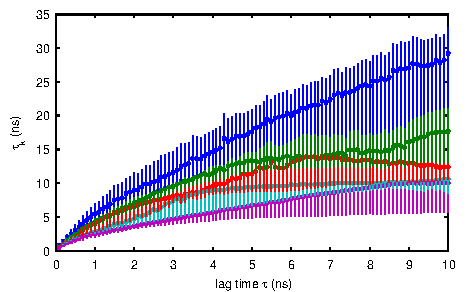
\includegraphics{chapters/automatic-state-decomposition/figures/Fs-peptide/Fs-timescales.pdf}}    
  \end{center}
  \caption{{\bf Implied timescales of the F$_s$ peptide as a function of lag time for 20-state automatic state decomposition.} 
   The five longest timescales are shown.  
   Circles represent the maximum likelihood estimate, and vertical bars depict 68\% symmetric confidence intervals about the mean.
   Note the timescales associated with two processes appear to cross, but are here colored and uncertainties are estimated with bootstrapping by ordering them by rank.
   This may cause the uncertainties depicted here to be an underestimate of the true uncertainties of each process.
  }
  \label{figure:fs-peptide-timescales}
\end{figure}

We then examined the implied timescales as a function of lag time (Figure \ref{figure:fs-peptide-timescales}).
%In the first iteration of microstates, all the largest timescales increased with lag time, with the longest timescale rising from 2.5 ns at 500 ps lag time to 10 ns at 10 ns lag time.  
%The timescales between the split microstates and lumped macrostates were extremely similar through all the iterations.  
%By the end of the tenth iteration, many of the timescales leveled off by a lag time of 3-5ns.  However, some timescales did continue to rise over the range of lag times -- a signature of non-Markovian behavior.  
%In particular, the longest timescale rose from 3 ns at 500 ps lag time to 30 ns at 10 ns lag time. [FIGURE - show the lifetimes versus lag time at iteration 10-merged]
Lumping appeared to preserve the longest timescales found in the microstate transition matrix (data not shown), indicating that our lumping scheme had been successful in identifying a nondestructive lumping into kinetically metastable states at each iteration.
%Over the course of 10 iterations, the longest timescale (as assessed with a lag time of 10 ns) increased from 10 to 30 ns, suggesting that the iterative refinement was actually improving the quality of the state decomposition.
% JDC: Can we also give the metastabilities vs iteration?  That might be a nice way to summarize improvement.
% NS: I like that -- I'm going to report it at 100 ps since that's the lag time for which we're actually maximizing it
% NS: 1st iteration -- lag time of 100ps, Q = 12.5358, lag time of 10 ns, Q = 2.2949
% NS: 10th iteration -- lag time of 100ps, Q = 14.5024, lag time of 10 ns, Q = 4.3512
% NS added:
Over the course of 10 iterations, the metastability (as optimized with a lag time of 100 ps) increased from $12.5 \pm 0.3$ to $14.5 \pm 0.1$, suggesting that the iterative refinement was actually improving the quality of the state decomposition.
% NS deleted since this doesn't really seem true when looking at the figure.
%On the first iteration, the longest timescales increase nearly linearly with lag time, while on the last iteration, most timescales became stable by a lag time of 10 ns, suggesting that Markovian behavior had been achieved.
On the first iteration, the longest timescales increase nearly linearly with lag time, while on the last iteration, some of the longest timescales become stable by a lag time of 4 -- 5 ns, suggesting Markovian behavior for some of the processes.

Using the interpretation of eigenvector components in terms of aggregate modes described in Section \ref{section:theory:markov-model-introduction}, the longest timescale was found to correspond to movement between the extended helix/coil state (state 1) and one of the twisted helix-turn-helix states (state 18) with only 500 members.  
We found, however, that state 18 appeared a small number of times in thirty trajectories, and over 450 times in a single trajectory.
% JDC: Nina -- is this right?
% NS: Yup, I wrote a script to count the number of conformations per trajectory for each state.  This was a particularly long trajectory, which is why I think we initially thought it was in more than one.
Further examination revealed that conformations belonging to this state were almost exclusively adjacent to conformations belonging to state 5, and structural comparison of conformations of these two states showed they were strikingly similar.
This suggests that slight conformational differences between conformations in states 18 and 5 allowed the $K$-medoid clustering algorithm to partition between these states in a splitting step, and since state 18 was mainly isolated in a single trajectory, its self-transition probability was maximized by \emph{not} lumping it with state 5, even though the two behaved in a similar kinetic fashion.
Indeed, when we manually lump states 18 and 5, the longest timescale, corresponding to transitions involving state 18, disappears, but the remaining timescales are all preserved (data not shown).
% JDC: Do we want to comment on the importance of having many effectively independent trajectory segments passing through the same state?
% NS: I feel this is covered pretty well in the end when we talk about the statistical inefficiency, no?

A second potential cause of the increase with lag time observed 
% NS changed: I feel we've sufficiently explained away the rise in the longest timescale and are now trying to explain the rise in the other timescales.
% in the longest timescale 
in some of the other long timescales
may be due to the finite length of trajectories.
If the state is long-lived, and occurs near the trajectory beginning or end, then it can be seen that the estimated self-transition probability $T_{ii}$ increases as a function of lag time.
This effect is most pronounced when a state occurs in very few trajectories, and appears to be mitigated when the state occurs in many trajectories at random times within the trajectory.
%We believe a second cause of the rising timescales with lag time is that the finite length of the trajectories causes end effects with increasing lag time, and these end effects are more pronounced in states with less sampling. % Fix me
% JDC: Elaborate on this.
          
In order to determine which states are poorly characterized, we estimated the number of statistically independent visits to each macrostate.
Since sequential samples from a single trajectory are temporally correlated, we computed the integrated autocorrelation time \cite{swope:1982a,janke:2002a} $\tau_{\mathrm{ac},i}$ for each macrostate $i$.
% NS changed so two sentences don't start "in the absence of"
% In the absence of statistical uncertainty, 
Ignoring statistical uncertainty, this correlation time is an upper bound on the equilibration time within a state; long-lived states will necessarily have long autocorrelation times, but trajectories trapped within them may contain many uncorrelated samples if the internal equilibration time is short.
In the absence of a convenient way to quantify the internal equilibration time for each state\footnote{There is some indication that consideration of restrictions of Markov chains to these macrostates may facilitate the computation of the internal equilibration time \cite{meerbach:2004a}.}, the autocorrelation time provides a better estimate of the appropriate timescale than the time to reach global equilibrium $\tau_{\mathrm{eq}}$.
%In order to determine which states may be poorly characterized, we attempted to estimate the number of statistically independent visits to each macrostate.
%We calculated the normalized fluctuation autocorrelation function $C_{ii}(t)$ for each state $i$
%\begin{eqnarray}
%C_{ii}(t) &=& \frac{\expect{\chi_i(0) \chi_i(t)} - \expect{\chi_i}^2}{\expect{\chi_i^2} - \expect{\chi_i}^2} \\
%           &=& \frac{T_{ii}(t) - p_i}{1 - p_i} .
%\end{eqnarray}
%where $T_{ii}(t)$ is the diagonal element of the transition probability matrix at time $t$ and $p_i$ is the equilibrium probability of state $i$.
%Expectations were estimated as averages over all trajectories, employing both stationarity and time-reversibility.
%This correlation function assumes the value of unity at $t = 0$, and decays to zero as the state occupied by the trajectories becomes decorrelated with this initial state occupation.
%The integrated autocorrelation time $\tau_i$ is a measure of the time required for decorrelation, and is given by
%\begin{eqnarray}
%\tau_i = \sum_{t=1}^T \left( 1-\frac{t}{T} \right) C_{ii}(t) . \label{equation:integrated-autocorrelation-time}
%\end{eqnarray}
As the correlation functions became statistically unreliable at times larger than 10 ns, a least squares linear fit to the log of the computed correlation function over the first 10 ns was used to estimate the tail at times greater than 10 ns, and this combined correlation function 
% NS added
was
integrated to obtain the autocorrelation time.
The effective number of independent samples for each state was then estimated by summing the number of independent samples from each trajectory (which are assumed independent), where the effective number of independent samples of state $i$ from trajectory $n$ is computed as  $N^\mathrm{eff}_{ni} \approx \min\{ 1, N_{ni} / g_i \}$, where $N_{ni}$ is the number of configurations from trajectory $n$ in state $i$, and $g_i = 1 + 2 \tau_{\mathrm{ac},i}$ is the statistical inefficiency of state $i$.

Computed state autocorrelation times are given in Table \ref{table:helix-states}.
For many states, the correlation time was 1 -- 2 ns, giving thousands of independent samples; however, for five states, including the four which were involved in the four longest timescales, the correlation times were between 10 and 50 ns, suggesting that the dataset contained less than 
% NS changed: If we give one independent sample per trajectory, the last four states have 67, 30, 26, and 47 independent samples respectively.  The other state with large correlation time (13) has 256 independent samples
50
%ten 
independent samples of these states.
Currently, in the automatic state decomposition algorithm, we try to reduce the statistical uncertainty in the transition matrix by limiting the expected population of each state to be greater than some minimum number of configurations.
Since the conformations appearing within some states may be highly correlated, the number of conformations within a state is not the best measure of how statistically well-determined its transition elements are; instead, it may be advantageous to place a lower limit on the effective number of independent visits to each state, which is far less than the number of configurations it contains.
Alternatively, it may be necessary to ensure better characterization of these states by conducting additional simulations from them, provided the equilibrium transition probabilities can still be computed.

% TIME EVOLUTION PLOT
\begin{figure}[tb]
  \begin{center}
    \resizebox{3.375in}{!}{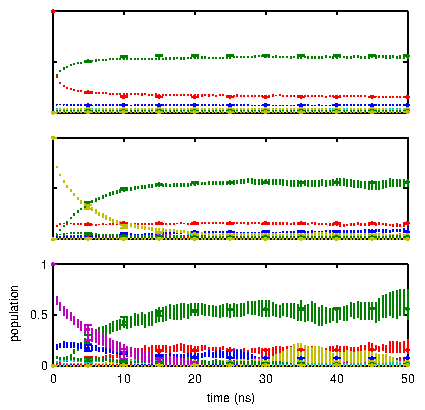
\includegraphics{chapters/automatic-state-decomposition/figures/Fs-peptide/fs-time-evolution.pdf}}    
  \end{center}
  \caption{{\bf Reproduction of observed state population evolution by Markov model for the F$_s$ peptide.} 
  The time evolution of the Markov model constructed from the 5 ns lag time transition matrix is shown by the filled circles with flat error bars, which denote the 68\% confidence interval from realizations of a bootstrap sample of 40 transition matrices computed from a 5 ns lag time.
  Vertical bars without flat ends denote the 68\% asymmetric confidence interval for the probability of finding the system in the 20 macrostates a given time after initial preparation in a specific state.
  The system was originally prepared in state 2 (top, red), 13 (middle, yellow), or 19 (bottom, purple).
  The most populous states are colored green (state 1), red (state 2), and blue (state 3).
  }
  \label{figure:fs-time-evolution}
\end{figure}

%Because of the difficulties described above, the models we were able to build for the F$_s$ peptide were not Markovian over reasonable timescales.
%However, our timescales corresponding to motion between well determined states, such as the extended helix/coil and bent helix/coil seem to be on the order of 5 -- 10 ns, which are not unreasonable given the extremely conservative estimate of full equilibration from an extremely biased starting conformation of 40 ns \cite{sorin:2005b}.
%We hope future versions of this algorithm will give shorter Markov times and shed more light on the kinetics of the F$_s$ peptide.
% JDC: COmmented this out.

We constructed a Markov model from the transition matrix estimated at a 5 ns lag time, where some (though apparently not all) of the timescales appear to have stabilized.
Repeated application of this transition matrix to an initial probability distribution can be compared to the transition probabilities at longer lag times estimated directly from the data to assess how well the model reproduces the observed kinetics.
The time evolution of probability density out of three states (state 2, a populous state; state 13, a moderately populated state; and state 19, a sparsely populated state) over the course of 50 ns is shown in Figure \ref{figure:fs-time-evolution}.
The Markov model appears to do a very reasonable job of predicting the time evolution of the system to within statistical uncertainty over many times longer than the lag time it was constructed for.
In fact, the time evolution was well-modeled for evolution out of nearly all states, except for state 13, for which dynamics seemed to be particularly poorly reproduced.
This state has a particularly long correlation time, and many trajectories seem to contain only a single configuration that is part of this state, suggesting its boundaries are simply poorly resolved.
Regardless, the time evolution is generally well-modeled for this system.

% Left from previous version, I don't think we need to do this -- Discuss whether the "star-like" trap states are artifacts of the sampling, force field, or actual states that are hard to observe experimentally.

% Old part left-over from previous version.  I don't think we can actually do this since the Markov time is too high compared with the overall equilibration time of the system.
    %Comparison with simulation data:
    %We eliminated the first 40 ns of simulation data, so the starting conformation of the trajectories was taken from an equilibrium distribution.
    %We selected those trajectories whose starting conformation was in a particular state, and plotted the state populations with time, for those trajectories.
    %We also calculated the state populations with time, given by the model propagated from a population of one of the given states.
    %(FIGURES of the comparison starting from different states)


